%-----------------------------------------------------------------------------%
\chapter{\babEmpat}
%-----------------------------------------------------------------------------%


Bab ini menjelaskan tentang perancangan sistem usulan, yaitu sistem rekomendasi lokasi pencacahan. Sebelum dijelaskan tentang sistem usulan, terlebih dahulu akan dilakukan eksperimen dan analisis terhadap solusi yang telah ada.


%-----------------------------------------------------------------------------%
\section{Analisis}
\label{sec:analysis}
%-----------------------------------------------------------------------------%
Pada kondisi saat ini (sistem berjalan), lokasi pencacahan sudah ditentukan sejak awal dengan menggunakan metode sampling tertentu. Pada tahap perancangan, sejumlah petugas direkrut dan ditugas pada sejumlah lokasi pencacahan. Pengalokasian seringkali dilakukan secara subjektif berdasarkan kedekatan lokasi pencacahan dengan domisili petugas pencacahan. Akibatnya, terjadi ketidakmerataan beban kerja dan variasi total waktu penyelesaian pekerjaan yang sangat tinggi antar petugas. 

Untuk mengatasi masalah ini, algoritma MDVRP dipilih karena memiliki karakteristik yang serupa dengan permasalahan alokasi petugas, yakni: 

\begin{enumerate}
	\item Terdapat lebih dari satu kendaraan, dimana masing-masing kendaraan memiliki depot yang berbeda. Hal ini analog dengan permasalahan alokasi petugas, dimana ada lebih dari satu pencacah dan tiap-tiap pencacah memiliki titik mulai pencacahan yang berbeda. 
	\item Terdapat biaya yang harus dikeluarkan untuk melakukan perjalanan dari satu pelanggan ke pelanggan yang lain. Ini sejalan dengan konsep dalam pencacahan dimana terdapat biaya untuk mengunjungi satu responden ke responden lainnya. 
\end{enumerate}

Pada proses pencacahan, biaya dapat berupa waktu tempuh, jarak tempuh, atau biaya perjalanan. Dalam penelitian ini, waktu tempuh dipilih sebagai representasi dari biaya karena waktu tempuh menggambarkan tingkat kesulitan akses dalam mengunjungi tiap-tiap wilayah kerja. Semakin sulit akses ke suatu wilayah, semakin lama waktu tempuh yang diperlukan. 

Eksperimen dilakukan untuk membuktikan fisibilitas algoritma MDVRP dalam penyelesaian permasalahan alokasi petugas. Eksperimen melibatkan 2 (dua) komponen utama:
\begin{enumerate}
	\item Sejumlah pencacah dengan depotnya masing-masing. 
	\item Sejumlah lokasi pencacahan/blok sensus yang setiap blok sensusnya memiliki beberapa responden. 
\end{enumerate}

\autoref{ssec:mtsp_dataset} hingga \autoref{ssec:hasil-analisis} menyajikan penjelasan rinci mengenai langkah-langkah yang dilakukan dalam eksperimen. 

%-----------------------------------------------------------------------------%
\subsection{Dataset}
\label{ssec:mtsp_dataset}
%-----------------------------------------------------------------------------%
\subsubsection{Lokasi Pencacahan}
%-----------------------------------------------------------------------------%
Merujuk kepada konsep MDVRP, lokasi pencacahan dapat dianalogikan sebagai pelanggan yang akan dikunjungi oleh petugas pencacahan (kendaraan). Pengujian dilakukan dengan menggunakan data 182 lokasi nagari/kelurahan yang bersumber dari data wilayah administratif di Kabupaten Pesisir Selatan, Provinsi Sumatera Barat. Masing-masing lokasi memiliki atribut ID dan posisi koordinat menurut garis lintang dan bujur, seperti yang terlihat pada \autoref{tbl:enumeration_locations}.


\begin{table*}[!]
	\centering
	\ra{1.3}
	\captionsetup{format=hang}
	\caption{Lokasi Pencacahan}
	\label{tbl:enumeration_locations}
	\begin{tabular}{lcc}
		\toprule
		& \multicolumn{2}{c}{Koordinat}\\
		\cmidrule{2-3}
		& Lintang & Bujur\\ 
		\midrule
		1302011001 & -2.3504 & 101.1434\\ 
		1302011002 & -2.4233 & 101.0285\\ 
		1302011003 & -2.3798 & 101.0427\\ 
		1302011004 & -2.3884 & 101.049\\ 
		1302011005 & -2.3936 & 101.0546\\
		...\\
		1302110019 & -1.2387 & 100.4853\\ 
		1302110020 & -1.1408 & 100.4938\\ 
		1302110021 & -1.0883 & 100.4652\\ 
		1302110022 & -1.0886 & 100.489\\ 
		1302110023 & -1.1523 & 100.4978\\
		\bottomrule
	\end{tabular}
\end{table*}


%-----------------------------------------------------------------------------%
\subsubsection{Petugas Pencacahan}
%-----------------------------------------------------------------------------%
Berdasarkan konsep MDVRP, petugas pencacahan diibaratkan sebagai kendaraan yang harus berpindah dari satu lokasi ke lokasi lain secara berurutan. Selain memiliki atribut ID, masing-masing pencacah juga dilengkapi dengan atribut depot, yaitu lokasi dimana pencacah harus memulai dan mengakhiri kunjungan. Eksperimen ini menggunakan 15 pencacah dengan lokasi depot yang bervariasi, seperti contoh yang tercantum pada \autoref{tbl:enumerator}.


\begin{table*}[!]
	\centering
	\ra{1.3}
	\captionsetup{format=hang}
	\caption{Pencacah}
	\label{tbl:enumerator}
	\begin{tabular}{lcc}
		\toprule
		& \multicolumn{2}{c}{Koordinat Depot}\\
		\cmidrule{2-3}
		& Lintang & Bujur\\ 
		\midrule
		1302011008 & -2.3905 & 101.1214\\
		1302012003 & -2.199 & 101.1188\\
		1302020006 & -2.1225 & 101.0687\\
		...\\
		1302100002 & -1.23265 & 100.54314\\
		1302101005 & -1.19831 & 100.58078\\
		1302110003 & -1.2475 & 100.4745\\
		\bottomrule
	\end{tabular}
\end{table*}


%-----------------------------------------------------------------------------%
\subsubsection{Jarak dan Waktu Tempuh}
\label{ss:distance-duration-matrix}
%-----------------------------------------------------------------------------%
Jarak dan waktu tempuh antar lokasi pencacahan digunakan sebagai penimbang dalam penentuan rekomendasi lokasi. Penghitungan jarak dan waktu tempuh dapat dilakukan dengan cara manual (menggunakan hasil survei lokasi dan perkiraan \textit{subject matter}) atau memanfaatkan \textit{Google Directions API} \citep{google_google_2016}. 


Secara teknis, \textit{Google Direction API} lebih unggul dibandingkan metode manual karena secara otomatis memperhitungkan faktor rute tercepat, kondisi geografis, moda transportasi yang digunakan, dan kemacetan lalu lintas dalam memperkirakan jarak dan waktu tempuh. Namun, \textit{Google Direction API} mengandalkan kontribusi para pengguna \textit{Google} sebagai sumber informasi, sehingga ada kemungkinan rute-rute yang jarang dilewati akan memiliki informasi yang minim dan cenderung bias. Sebagai konsekuesinya, terdapat resiko hasil kalkukasi yang kurang tepat untuk rute-rute tersebut. 


Kode \ref{lst:google_direction_api_request} menggambarkan contoh \textit{requests URL} yang dikirimkan ke \textit{Google Direction API}. \textit{Request URL} ini dapat dieksekusi dengan menggunakan \textit{HTTP client}, seperti \textit{curl} dan \textit{wget}, atau \textit{HTTP client library}, seperti \textit{requests} dan \textit{urllib} di Python. Contoh \textit{response} Google Direction API dapat dilihat pada \autoref{fig:google_direction_api_response}.


Hasil kalkulasi jarak dan waktu tempuh kemudian disimpan dalam bentuk matriks seperti yang terlihat pada Tabel \ref{tbl:distance_duration_matrix}. Jika lokasi depot dari pencacah tidak tercakup dalam lokasi pencacahan yang ada, maka lokasi depot tersebut harus ditambahkan ke dalam matriks jarak dan waktu tempuh.


\begin{listing}[!]
	\captionsetup{format=hang}
	\caption{\textit{Google Direction API Request}}
	\label{lst:google_direction_api_request}
	\begin{minted}[showspaces=false, breaklines=true]{http}
https://maps.googleapis.com/maps/api/directions/json?origin=origin_lat,
origin_lon&destination=dest_lat,dest_lon&departure_time=timestamp&
traffic_model=best_guess&key=API_KEY
	\end{minted}
\end{listing}


\begin{figure}[!]
	\centering
	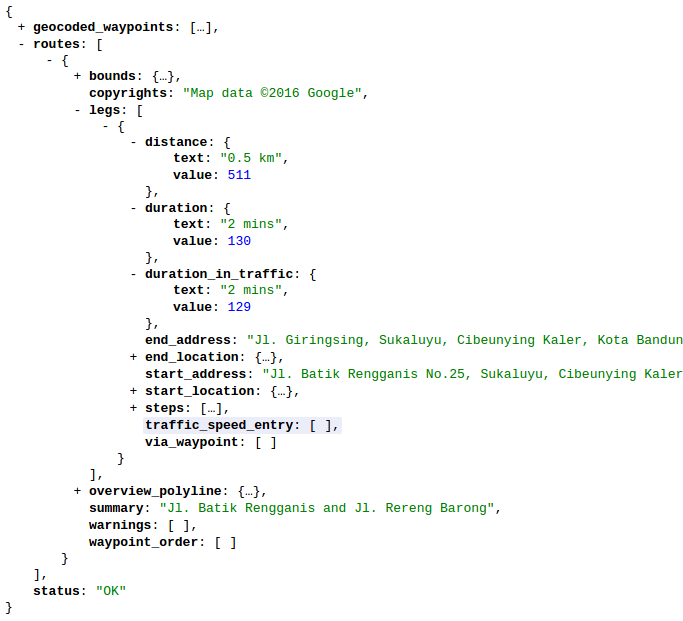
\includegraphics[width=\textwidth]{Resources/Images/google_direction_api_response}
	\captionsetup{format=hang}
	\caption{\textit{Google Direction API Response}}
	\label{fig:google_direction_api_response}
\end{figure}


\begin{table}[!]
	\centering
	\ra{1.3}
	\captionsetup{format=hang}
	\caption{Data Jarak dan Waktu Tempuh}
	\label{tbl:distance_duration_matrix}
	\begin{tabular}{llcc}
		\toprule
		Lokasi A & Lokasi B & Jarak (m) & Waktu Tempuh (det)\\
		\midrule
		1302021001 & 1302021003 & 11119 & 1055\\
		1302021001 & 1302021002 & 9373 & 868\\
		1302021001 & 1302021005 & 490 & 38\\
		1302021001 & 1302021004 & 22760 & 2044\\
		...\\
		1302040015 & 1302012010 & 77889 & 8305\\
		1302040014 & 1302100015 & 103893 & 9984\\
		1302040014 & 1302012010 & 73561 & 7546\\
		1302100015 & 1302012010 & 171636 & 16801\\
		\bottomrule
	\end{tabular}
\end{table}


%-----------------------------------------------------------------------------%
\subsection{Algoritma dan Implementasi}
\label{ssec:alg-impl}
%-----------------------------------------------------------------------------%
Terdapat banyak \textit{library} yang dapat digunakan untuk mengatasi permasalahan MDVRP, baik yang berbayar maupun \textit{open source}. Dua \textit{open source library} yang cukup banyak digunakan untuk menyelesaikan permasalahan MDVRP adalah Jsprit \citep{jsprit_jsprit_2014} dan Optaplanner \citep{optaplanner_constraint_2016}. Eksperimen ini menggunakan JSprit karena JSprit lebih berfokus pada pencarian rute serta lebih mudah untuk diimplementasikan. 


Jsprit merupakan sebuah library berbasis java yang digunakan untuk menyelesaikan permasalahan \textit{traveling salesman problem} (TSP) dan \textit{vehicle routing problems} (VRP). JSprit mencakup berbagai skenario seperti: \textit{pickups and deliveries}, \textit{back hauls}, \textit{heterogeneous fleets}, \textit{finite and infinite fleets}, \textit{multiple depots}, \textit{time windows}, \textit{open routes}, \textit{different start and end locations}, \textit{multiple capacity dimensions}, \textit{initial loads}, dan \textit{skills}. JSpirit bekerja secara terstruktur, mulai dari pendefinisan masalah, pemilihan algoritma, pencarian solusi, hingga pemilihan solusi terbaik.


%-----------------------------------------------------------------------------%
\subsubsection{Definisi Masalah}
%-----------------------------------------------------------------------------%
Pendefinisian masalah dengan \textit{library} Jsprit dilakukan dengan mendefinisikan lokasi pencacahan, para pencacah, dan matriks jarak dan waktu tempuh yang diimplementasikan dalam Kode \ref{lst:jsprit_define_locations}, Kode \ref{lst:jsprit_define_enumerators}, dan Kode \ref{lst:jsprit_define_route_weights}. Ketiga variabel ini kemudian di-\textit{build} menjadi satu dengan menggunakan \textit{syntax} yang tercantum pada Kode \ref{lst:jsprit_build_problem}.


\begin{listing}[!]
	\captionsetup{format=hang}
	\caption{Definisi Lokasi Pencacahan}
	\label{lst:jsprit_define_locations}
	\begin{minted}[showspaces=false,breaklines=true]{java}
Service.Builder builder = Service.Builder.newInstance(line[0]);

try {
	Location loc = Location.Builder.newInstance()
		.setId(line[0])
		.setCoordinate(
	Coordinate.newInstance(Double.parseDouble(line[2]), 
	Double.parseDouble(line[1]))).build();
	builder.setLocation(loc);
} catch (Exception e) {}

Service node = builder.build();
vrpBuilder.addJob(node);
	\end{minted}
\end{listing}


\begin{listing}[!]
	\captionsetup{format=hang}
	\caption{Definisi Pencacah dari File .csv}
	\label{lst:jsprit_define_enumerators}
	\begin{minted}[showspaces=false,breaklines=true]{java}
VehicleTypeImpl.Builder vehicleTypeBuilder = VehicleTypeImpl.Builder.newInstance("enumerator");
vehicleTypeBuilder.setCostPerDistance(0);
vehicleTypeBuilder.setCostPerTransportTime(1);
vehicleTypeBuilder.setCostPerServiceTime(1);
VehicleType vehicleType = vehicleTypeBuilder.build();

VehicleImpl.Builder builder = VehicleImpl.Builder.newInstance(line[0]);

try {
	Location loc = Location.Builder.newInstance()
		.setId(line[0])
		.setCoordinate(Coordinate.newInstance(
			Double.parseDouble(line[2]), Double.parseDouble(line[1])))
		.build();
	builder.setStartLocation(loc);
} catch (Exception e) {}


builder.setType(vehicleType);
VehicleImpl vehicle = builder.build();
vrpBuilder.addVehicle(vehicle);
	\end{minted}
\end{listing}


\begin{listing}[!]
	\captionsetup{format=hang}
	\caption{Definisi Penimbang Jarak dan Waktu Tempuh dari File .csv}
	\label{lst:jsprit_define_route_weights}
	\begin{minted}[showspaces=false,breaklines=true]{java}
VehicleRoutingTransportCostsMatrix.Builder costMatrixBuilder = VehicleRoutingTransportCostsMatrix.Builder.newInstance(true);

while ((line = reader.readNext()) != null) {
	try {
		costMatrixBuilder.addTransportDistance(line[0], line[1], Double.parseDouble(line[2]));
		costMatrixBuilder.addTransportTime(line[0], line[1], Double.parseDouble(line[3]));
	} catch (Exception e) {
		costMatrixBuilder.addTransportDistance(line[0], line[1], 0.0);
		costMatrixBuilder.addTransportTime(line[0], line[1], 0.0);
	}
}

VehicleRoutingTransportCosts costMatrix = costMatrixBuilder.build();
vrpBuilder.setRoutingCost(costMatrix);
	\end{minted}
\end{listing}


\begin{listing}[!]
	\captionsetup{format=hang}
	\caption{Pendefinisian Masalah}
	\label{lst:jsprit_build_problem}
	\begin{minted}[showspaces=false,breaklines=true]{java}
VehicleRoutingProblem.Builder vrpBuilder = VehicleRoutingProblem.Builder.newInstance();
vrpBuilder.setFleetSize(VehicleRoutingProblem.FleetSize.FINITE);
VehicleRoutingProblem problem = vrpBuilder.build();
	\end{minted}
\end{listing}


%-----------------------------------------------------------------------------%
\subsubsection{Konfigurasi Algoritma}
%-----------------------------------------------------------------------------%
Berdasarkan masalah yang telah didefinisikan sebelumnya, JSprit kemudian akan membuat konfigurasi algoritma. Secara \textit{default} algoritma yang digunakan adalah \textit{Tabu Search}. Selain itu, jumlah iterasi dan \textit{thread} yang digunakan juga dapat didefinisikan. Kode \ref{lst:jsprit_create_algorithm} merupakan \textit{syntax} konfigurasi algoritma yang digunakan. 


\begin{listing}[!]
	\captionsetup{format=hang}
	\caption{Penentuan Algoritma}
	\label{lst:jsprit_create_algorithm}
	\begin{minted}[showspaces=false,breaklines=true]{java}
	VehicleRoutingAlgorithm algorithm = Jsprit.Builder.newInstance(problem)
	.setProperty(Jsprit.Parameter.THREADS, 5).buildAlgorithm();
	algorithm.setMaxIterations(iterations);
	\end{minted}
\end{listing}


%-----------------------------------------------------------------------------%
\subsubsection{Pencarian Solusi dan Penentuan Solusi Terbaik}
%-----------------------------------------------------------------------------%
Pencarian solusi dilakukan dengan menggunakan algoritma yang didefinisikan pada tahap sebelumnya. Jika algoritma memproduksi lebih dari satu solusi, maka Jspirit akan melakukan pemilihan solusi terbaik seperti yang terlihat pada Kode \ref{lst:jsprit_search_solution}. Secara \textit{default}, solusi terbaik merupakan solusi yang memiliki total biaya terrendah.


\begin{listing}[!]
	\captionsetup{format=hang}
	\caption{Pencarian Solusi}
	\label{lst:jsprit_search_solution}
	\begin{minted}[showspaces=false,breaklines=true]{java}
	Collection<VehicleRoutingProblemSolution> solutions = algorithm.searchSolutions();
	VehicleRoutingProblemSolution bestSolution = Solutions.bestOf(solutions);
	\end{minted}
\end{listing}


%-----------------------------------------------------------------------------%
\subsection{Hasil dan Analisis}
\label{ssec:hasil-analisis}
%-----------------------------------------------------------------------------%
Berdasarkan hasil dari eksperimen, diperoleh rute seperti yang digambarkan pada Gambar \ref{fig:analysis_mtsp_recommendation} dan Listing \ref{lst:analysis_mtsp_recommendation} untuk detail dari setiap pencacah. Berdasarkan rute tersebut kemudian dilakukan simulasi pencacahan dengan menyertakan waktu tempuh dan lama pencacahan pada tiap-tiap lokasi. Lama pencacahan untuk tiap-tiap lokasi pencacahan dibuat dengan mengikuti distribusi normal. Pengujian dengan menggunakan 182 lokasi pencacahan dan 15 petugas pencacahan menghasilkan rata-rata dan standar deviasi waktu penyelesaian tugas sebesar:  
$$ \mu = 82,24 jam $$
$$ \sigma = 88,95 jam $$


\begin{figure}[!]
	\centering
	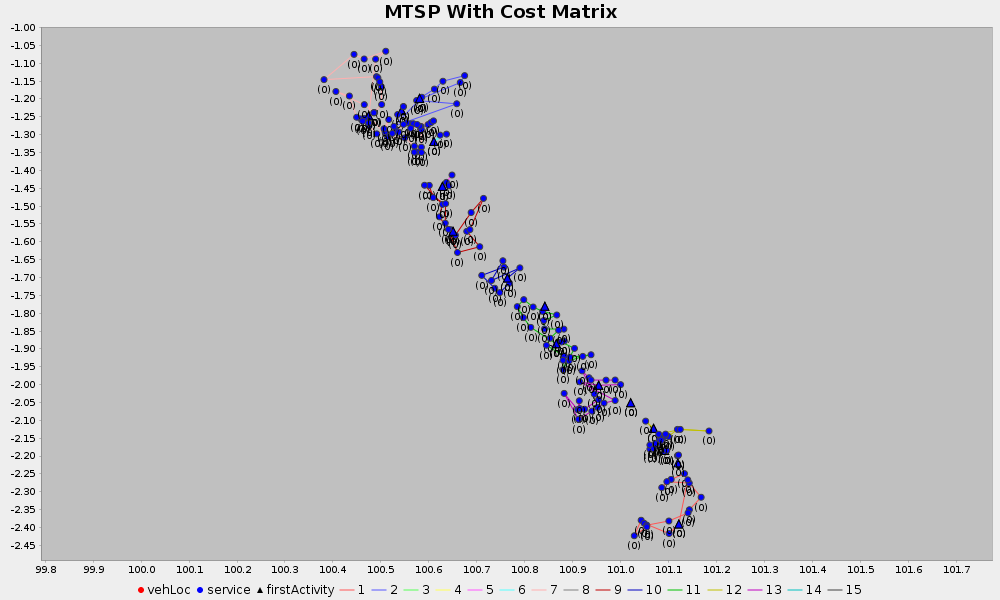
\includegraphics[width=\textwidth]{Resources/Images/analysis_mtsp_no_time_windows}
	\captionsetup{format=hang}
	\caption{Rute yang dihasilkan oleh JSprit}
	\label{fig:analysis_mtsp_recommendation}
\end{figure}


\begin{listing}[!]
	\captionsetup{format=hang}
	\caption{Detail rute yang dihasilkan oleh JSprit}
	\label{lst:analysis_mtsp_recommendation}
	\begin{minted}[showspaces=false,breaklines=true, escapeinside=||]{text}
|\textbf{1302021005}| : 1302021001 --> 1302021005
|\textbf{1302101005}| : 1302101005 --> 1302101001 --> 1302100010 --> 1302100014 --> 1302100011 --> 1302101004 --> 1302101006 --> 1302101003 --> 1302101002
|\textbf{1302070006}| : 1302070006 --> 1302070002 --> 1302070003 --> 1302080009 --> 1302080004 --> 1302080001 --> 1302080005 --> 1302080003 --> 1302070012 --> 1302070011 --> 1302070001 --> 1302070004 --> 1302070007 --> 1302070008 --> 1302070010 --> 1302070009 --> 1302070005
|\textbf{1302050007}| : 1302050007
|\textbf{1302100002}| : 1302100002 --> 1302100003 --> 1302100013 --> 1302100012
|\textbf{1302030005}| : 1302030005
|\textbf{1302110003}| : 1302110003 --> 1302100001 --> 1302090006 --> 1302090012 --> 1302090003 --> 1302090014 --> 1302090009 --> 1302090015 --> 1302090018 --> 1302090016 --> 1302090017 --> 1302090013 --> 1302090005 --> 1302090007 --> 1302090002 --> 1302090008 --> 1302090001 --> 1302100015 --> 1302100004 --> 1302100016 --> 1302090011 --> 1302090010 --> 1302100017 --> 1302100006 --> 1302100007 --> 1302100009 --> 1302100008 --> 1302100005 --> 1302110001 --> 1302110010 --> 1302110013 --> 1302110002 --> 1302110014 --> 1302110015 --> 1302110011 --> 1302110016 --> 1302110017 --> 1302110004 --> 1302110018 --> 1302110019 --> 1302110005 --> 1302110012 --> 1302110023 --> 1302110020 --> 1302110006 --> 1302110007 --> 1302110008 --> 1302110021 --> 1302110009 --> 1302110022
|\textbf{1302012003}| : 1302012007 --> 1302012003 --> 1302012008
|\textbf{1302080006}| : 1302080006 --> 1302080008 --> 1302080002 --> 1302080007
|\textbf{1302031005}| : 1302031005 --> 1302031008 --> 1302030014 --> 1302030006 --> 1302030009 --> 1302030004 --> 1302030010 --> 1302031003 --> 1302030002 --> 1302031004 --> 1302030003 --> 1302030012 --> 1302031001 --> 1302031006 --> 1302040011 --> 1302031009 --> 1302031010 --> 1302031002 --> 1302031007 --> 1302030001
|\textbf{1302060005}| : 1302060005 --> 1302060009 --> 1302060006 --> 1302060008 --> 1302060002 --> 1302060007 --> 1302060001 --> 1302060003 --> 1302060004
|\textbf{1302020006}| : 1302020006 --> 1302020015 --> 1302020011 --> 1302020009 --> 1302020010 --> 1302020001 --> 1302020003 --> 1302020005 --> 1302021006 --> 1302021002 --> 1302021007 --> 1302021008 --> 1302021003 --> 1302021009 --> 1302021004 --> 1302021010 --> 1302020016 --> 1302020017
|\textbf{1302011008}| : 1302011008 --> 1302011007 --> 1302011004 --> 1302011003 --> 1302011002 --> 1302011006 --> 1302011005 --> 1302011009 --> 1302011010 --> 1302011001 --> 1302012005 --> 1302012002 --> 1302012009 --> 1302012010 --> 1302012004 --> 1302012001 --> 1302012006
|\textbf{1302040002}| : 1302040002 --> 1302040003 --> 1302040004 --> 1302040015 --> 1302040008 --> 1302040009 --> 1302040010 --> 1302040014 --> 1302040012 --> 1302040013 --> 1302040001 --> 1302040016 --> 1302040007 --> 1302040006 --> 1302040005 --> 1302050001 --> 1302050004 --> 1302050006 --> 1302050002 --> 1302050008 --> 1302050010 --> 1302050009 --> 1302050005 --> 1302050003
|\textbf{1302090004}| : 1302090004 --> 1302090019 --> 1302090020
	\end{minted}
\end{listing}


\begin{table}[!]
	\centering
	\ra{1.3}
	\captionsetup{format=hang}
	\caption{Waktu total dari setiap rute yang dihasilkan oleh JSprit}
	\label{tbl:enumerators_total_time}
	\begin{tabular}{lc}
		\toprule
		Pencacah & Total Waktu (jam)\\
		\midrule
		1302021005 & 13.3\\
		1302101005 & 60.8\\
		1302070006 & 116\\
		1302050007 & 6\\
		1302100002 & 26.6\\
		1302030005 & 6\\
		1302110003 & 341\\
		1302012003 & 19.9\\
		1302080006 & 27.1\\
		1302031005 & 136\\
		1302060005 & 61.3\\
		1302020006 & 121\\
		1302011008 & 116\\
		1302040002 & 162\\
		1302090004 & 20.2\\
		\bottomrule
	\end{tabular}
\end{table}


Nilai standar deviasi yang tinggi menunjukkan terjadinya ketidakmerataan beban kerja antar pencacah. Ini sekaligus menunjukkan bahwa algoritma MDVRP murni kurang ideal untuk digunakan dalam penentuan rekomendasi. Hal ini terjadi karena algoritma MDVRP memproduksi solusi berupa \textit{precalculated routes} (rute yang harus dikunjungi dari awal hingga akhir tugas pencacahan) tanpa memperhitungkan faktor lamanya waktu kunjungan pada satu lokasi pencacahan. Variabel lama waktu pencacahan hanya akan tersedia jika suatu lokasi sudah selesai dikunjungi sehingga tidak bisa diikutsertakan dalam kalkulasi rekomendasi. \autoref{fig:illustration-timeline-mdvrp-no-service-time} menunjukkan ilustrasi ketidaksesuaian penggunaan algoritma MDVRP murni pada permasalahan alokasi petugas pencacahan yang dapat dijabarkan sebagai berikut:
\begin{enumerate}
	\item Terdapat 10 lokasi pencacahan yang harus dikunjungi. algoritma MDVRP menciptakan solusi berupa \textit{precalculated routes} untuk petugas A dan B, dimana masing-masing mendapatkan jumlah beban tugas yang sama besar, yakni 5 lokasi. Pada tahap ini, petugas A dan B sama-sama sudah mengetahui urutan lokasi yang akan mereka kunjungi dari awal hingga akhir kegiatan pencacahan. 
	\item Petugas pencacahan A dan B sama-sama memulai tugas pada waktu $t_{s}$ (\textit{time start}) yang digambarkan sebagai segmen berwarna hijau.
	\item Petugas A dan B mengunjungi lokasi pencacahan masing-masing (lokasi \textit{i}) yang memakan waktu selama $t_{i}$ (segmen berwarna putih). Perlu diingat bahwa lokasi $i$ yang dituju oleh petugas A berbeda dengan lokasi $i$ yang dituju oleh petugas B.
	\item Pada setiap lokasi $i$, baik petugas A maupun petugas B memerlukan waktu sebesar $t_{i.1}$ untuk menyelesaikan tugas pencacahan (segmen berwarna biru).  
	\item Petugas A dan B menyelesaikan tugas pada waktu $t_{f}$ (\textit{time finish}) yang digambarkan sebagai segmen berwarna merah muda. 
\end{enumerate}

Dari \autoref{fig:illustration-timeline-mdvrp-no-service-time}, terlihat bahwa kalkulasi rekomendasi rute tanpa melibatkan lama pencacahan mengakibatkan $t_{i}$ dan $t_{i.1}$ yang tidak setara antara petugas A dan B. Hal ini terlihat dari posisi $t_{f}$ petugas A yang jauh berbeda dengan posisi $t_{f}$ petugas B pada \textit{timeline} masing-masing. Petugas A mendapatkan rute dengan rata-rata \textit{service time} ($t_{i.1}$) yang lebih panjang sehingga $t_{f}$ petugas A menjadi lebih besar dibandingkan $t_{f}$ petugas B. Perbedaan yang paling signifikan terlihat pada lokasi pencacahan kedua ($i = 2$) dimana petugas A memiliki $t_{2.1}$ yang hampir 3 (tiga) kali lebih besar dari $t_{2.1}$ petugas B. Sebagai dampaknya, terjadi ketimpangan dalam total waktu penyelesaian pencacahan antar petugas, dimana beban tugas petugas A menjadi jauh lebih berat dibandingkan petugas B. 

\begin{figure}[!]
	\centering
	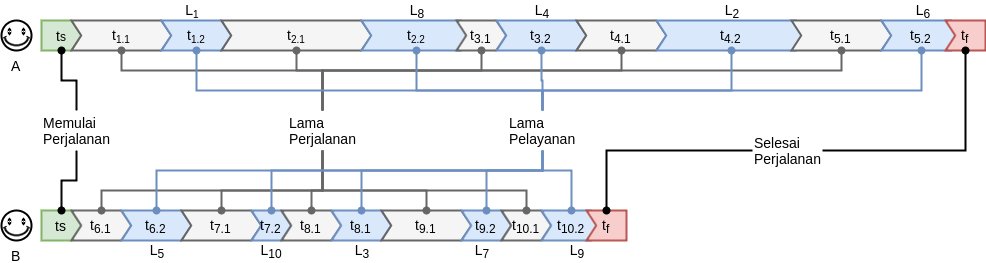
\includegraphics[width=\textwidth]{Resources/Images/illustration-timeline-mdvrp}
	\caption{Ilustrasi \textit{Timeline} Rute yang Dikalkulasi Tanpa Melibatkan Waktu Pencacahan}
	\label{fig:illustration-timeline-mdvrp-no-service-time}
\end{figure}


Untuk mengatasi masalah ini diperlukan suatu mekanisme kalkulasi rekomendasi yang tidak terikat pada lama waktu pencacahan. Mekanisme ini kemudian akan dikombinasikan dengan algoritma MDVRP sehingga menghasilkan suatu metode baru yang dapat menutupi kelemahan MDVRP sekaligus memberikan rekomendasi rute yang lebih adil kepada semua petugas pencacahan. 


%-----------------------------------------------------------------------------%
\section{Perancangan Solusi}
\label{sec:design}
%-----------------------------------------------------------------------------%
Hasil eksperimen pada \autoref{ssec:hasil-analisis} menunjukkan bahwa mekanisme kalkulasi yang bebas dari `lama pencacahan' diperlukan untuk menghilangkan bias dan kesenjangan rute untuk tiap-tiap petugas. Solusi yang diusulkan untuk mengatasi masalah ini adalah dengan melakukan penghitungan rute secara bertahap dengan melakukan `hibridisasi' antara algoritma MDVRP dengan suatu mekanisme \textit{real time}. Idenya adalah, alih-alih menghitung rute secara lengkap diawal pencacahan, lebih baik rute dihitung secara bertahap secara \textit{real time} dengan memanfaatkan `lokasi terkini' dari petugas sebagai depot yang baru pada setiap tahapnya. Pada saat awal pencacahan, petugas hanya mengetahui lokasi pertama yang akan mereka kunjungi. Setelah menyelesaikan tugas pencacahan pada lokasi tersebut, petugas harus mengirimkan permintaan ke \textit{server} guna mengetahui lokasi pencacahan berikutnya.

\autoref{fig:illustration-timeline-realtime-mdvrp} menggambarkan penerapan \textit{real time} MDVRP untuk mengatasi permasalahan alokasi petugas pencacahan yang dijabarkan sebagai berikut:
\begin{enumerate}
	\item Terdapat 10 lokasi pencacahan yang harus dikunjungi. Petugas pencacahan A dan B sama-sama memulai tugas pada waktu $t_{s}$ (segmen berwarna hijau). Berbeda dengan mekanisme pada \autoref{fig:illustration-timeline-mdvrp-no-service-time}, pada tahap ini, petugas A dan B sama-sama tidak memiliki pengetahuan apapun tentang urutan lokasi yang harus mereka kunjungi. 
	\item Pada waktu $t_{1}$ (segmen berwarna kuning), A dan B mengirimkan permintaan ke \textit{server} untuk mendapatkan lokasi pertama yang harus mereka kunjungi. 
	\item A dan B berjalan menuju lokasi pencacahan masing-masing (lokasi \textit{i}) yang memerlukan waktu tempuh sebesar $t_{i.1}$ (segmen berwarna putih). Lokasi $i$ yang dituju oleh petugas A berbeda dengan lokasi $i$ yang dituju oleh petugas B.
	\item A dan B menyelesaikan tugas pencacahan di lokasi pertama yang menghabiskan waktu sebesar $t_{i.2}$ (segmen berwarna biru).
	\item Setelah menyelesaikan tugas di lokasi pertama, A dan B mengirimkan \textit{request} ke server untuk mengetahui lokasi berikutnya yang harus dikunjungi. Server kemudian melakukan rekalkulasi rute dengan melakukan pengecekan terhadap 8 lokasi yang belum dikunjungi dan mencocokkannya dengan `lokasi terkini' dari petugas. Lokasi pencacahan berikutnya yang merupakan lokasi terbaik jika dihitung dari `lokasi terkini', akan dikirimkan sebagai balasan terhadap permintaan yang telah dikirimkan oleh petugas. 
	\item A dan B melanjutkan tugas pencacahan ke lokasi berikutnya (lokasi $i = 2$), dimana setiap lokasi memerlukan waktu tempuh sebesar $t_{i.1}$ dan waktu penyelesaian pencacahan (\textit{service time}) sebesar $t_{i.2}$. Proses pada poin 2 hingga 6 akan terus berulang hingga seluruh lokasi target pencacahan selesai dikunjungi. 
	\item Petugas A dan B menyelesaikan tugas pada waktu $t_{f}$ (segmen berwarna merah muda) yang hampir sama. Dari \autoref{fig:illustration-timeline-realtime-mdvrp} terlihat bahwa jumlah lokasi yang dikunjungi oleh petugas A lebih sedikit dibandingkan petugas B. Hal ini dikarenakan petugas A memerlukan waktu yang lebih lama untuk melakukan perjalanan ke lokasi serta menyelesaikan tugas pencacahan di lokasi tersebut. 
\end{enumerate}


Mayoritas \textit{real time system} diimplementasikan dengan menggunakan \textit{Web service}. Namun, sistem kerjanya yang \textit{synchronous} (\textit{request} dan \textit{reply} harus diproses secara berurutan) menyebabkan \textit{web service} tidak cocok digunakan untuk aplikasi yang bersifat \textit{information driven} \citep{muhl_large-scale_2002}. Sebagai alternatif, mekanisme \textit{publish/subscribe} dipilih karena memungkinkan terjadinya komunikasi yang \textit{asynchronous} antara \textit{server (publisher)} dan \textit{client (subscriber)}, dimana komunikasi tetap dapat berjalan walaupun salah satu pihak sedang dalam kondisi \textit{offline}.


\begin{figure}[!]
	\centering
	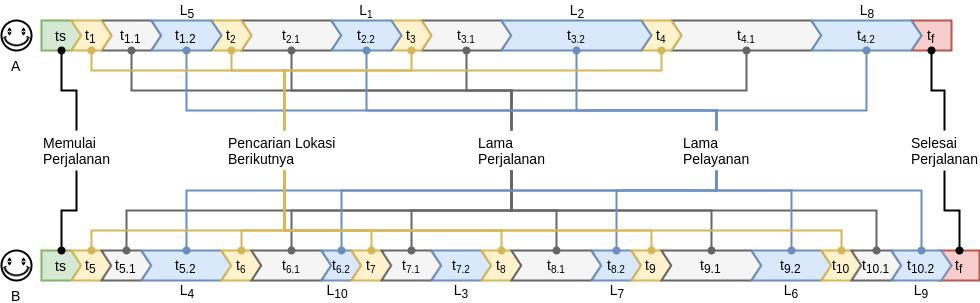
\includegraphics[width=\textwidth]{Resources/Images/illustration-timeline-realtime-mdvrp}
	\captionsetup{format=hang}
	\caption{Ilustrasi \textit{Timeline} Penerapan MDVRP Secara \textit{Real Time}}
	\label{fig:illustration-timeline-realtime-mdvrp}
\end{figure}

%-----------------------------------------------------------------------------%
\subsection{Garis Besar Sistem Usulan}
%-----------------------------------------------------------------------------%
Sistem usulan untuk rekomendasi lokasi pencacahan dirancang berdasarkan arsitektur \textit{publish/subscribe} yang terdiri dari 3 (tiga) komponen utama, yaitu: \textit{publisher} rekomendasi, petugas pencacahan yang berperan sebagai \textit{subscriber}, dan \textit{message broker} yang berperan sebagai penerus pesan (\textit{message router}). \autoref{fig:system-overview} memberikan ilustrasi komponen yang menyusun sistem rekomendasi lokasi pencacahan usulan.


\begin{figure}[!]
	\centering
	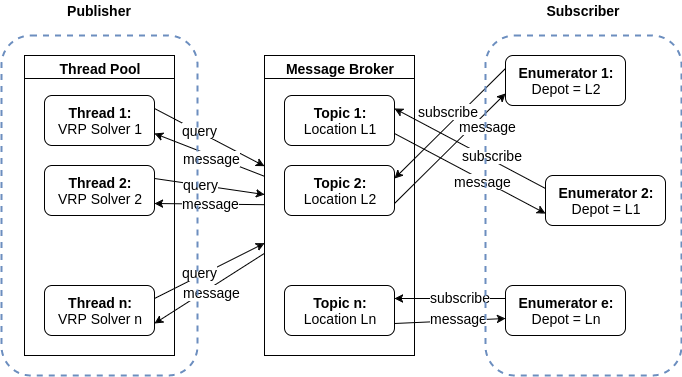
\includegraphics[width=\textwidth]{Resources/Images/system-overview}
	\captionsetup{format=hang}
	\caption{Garis Besar Sistem Usulan}
	\label{fig:system-overview}
\end{figure}


Komunikasi antara \textit{publisher} dan \textit{subscriber} terjadi atas dasar kesamaan topik (\textit{event}). Topik diperoleh dari konteks setiap pencacah yang dapat berupa jenis kelamin, tingkat pendidikan, umur, pengalaman, atau domisili/lokasi pencacah. Pada penelitian ini, `lokasi terkini' dari pencacah dipilih sebagai topik karena bersifat unik, dimana setiap lokasi pencacahan hanya akan dikunjungi oleh satu orang pencacah saja dan tidak akan ada lebih dari satu pencacah dengan `lokasi terkini' yang sama.


%-----------------------------------------------------------------------------%
\subsection{\textit{Publisher} Rekomendasi}
\label{ssec:publisher}
%-----------------------------------------------------------------------------%
Berdasarkan konsep dasar mekanisme \textit{publish/subscribe}, \textit{publisher} akan mengirimkan informasi ke seluruh \textit{subscriber} tanpa melihat apakah \textit{subscriber} tersebut memang men-\textit{subscribe} topik dari informasi yang bersangkutan atau tidak. Akibatnya informasi yang dikirim banyak yang tidak tepat sasaran sehingga komunikasi yang berlangsung menjadi tidak efisien. Untuk mengatasi inefisiensi komunikasi ini, perlu dilakukan beberapa penyesuaian agar \textit{publisher} hanya akan mengirimkan informasi kepada \textit{subscriber} yang bersesuaian. 

Pada saat seorang petugas pencacahan yang berperan sebagai \textit{subscriber} mengirimkan permintaan `lokasi pencacahan yang harus dituju' kepada \textit{publisher}, permintaan ini tidak langsung diterima oleh \textit{publisher}, melainkan ditampung oleh \textit{message broker}. \textit{Publisher} perlu mengecek \textit{message broker} secara berkala untuk mendeteksi ada atau tidaknya \textit{request} baru dengan menggunakan \textit{thread} $TopicWatcher$ yang dideskripsikan pada \autoref{alg:topic-watcher} serta digambarkan dengan \textit{flowchart} pada \autoref{fig:topic-watcher}. 


\begin{algorithm}[!]
	\captionsetup{format=hang}
	\caption{TopicWatcher}
	\label{alg:topic-watcher}
	\begin{algorithmic}[1]
		\renewcommand{\algorithmicrequire}{\textbf{Input:}}
		\renewcommand{\algorithmicensure}{\textbf{Output:}}
		\REQUIRE $None$
		\ENSURE  $None$
		\\ $TP$ = Threadpool
		\\ $N$ = Number of locations
		\\ $M$ = Number of enumerators
		\WHILE {true}
		\STATE $C \leftarrow readAvailableTopicFromBroker()$	// channel
		\FOR {$m = 1$ to $len(C)$}
		\FOR {$n = 1$ to $N$}
		\IF {($C_m == L_n$)}
		\STATE $T_n = Thread(C_m, E_1...E_M, (unassigned) L_1...L_N)$		// E = enumerator
		\STATE submitThreadToThreadpool($T_n$, $TP$)
		\ENDIF
		\ENDFOR
		\ENDFOR
		\ENDWHILE
	\end{algorithmic}
\end{algorithm}


\begin{figure}[!]
	\centering
	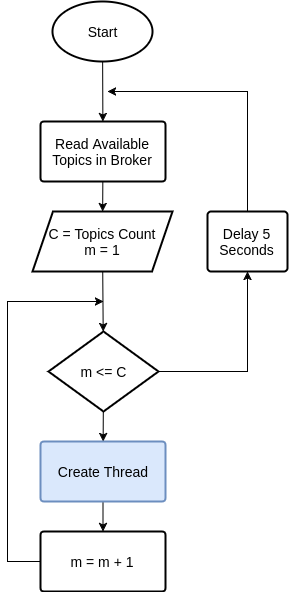
\includegraphics[width=6.3cm]{Resources/Images/topic-watcher}
	\captionsetup{format=hang}
	\caption{\textit{\textit{Flowchart} Topic Watcher}}
	\label{fig:topic-watcher}
\end{figure}


Untuk setiap permintaan yang diterima, \textit{publisher} akan menyiapkan sebuah \textit{thread} baru dengan menggunakan `lokasi terkini' dari \textit{subscriber} (petugas) sebagai ID. \textit{Thread} ini dilengkapi dengan sebuah $VRP solver procedure$ (\autoref{alg:vrp-worker}) yang akan melakukan pencarian solusi/rute. Seluruh \textit{thread} dari masing-masing topik ditampung di dalam sebuah \textit{threadpool} yang menangani \textit{thread} berdasarkan urutan waktu kedatangan. Pada akhir proses pencacahan ketika seluruh lokasi pencacahan telah dialokasikan kepada petugas, ukuran \textit{threadpool} ini akan sama dengan jumlah seluruh topik yang tersedia. 


\textit{Thread-thread} di dalam \textit{threadpool} dieksekusi satu per satu sesuai dengan waktu kedatangan. Setiap eksekusi akan melibatkan \textit{VRPSolver procedure} yang mengikutsertakan $M$ \textit{subscribers} (petugas pencacahan) dan \textit{unassigned} N lokasi pencacahan. \textit{VRPSolver procedure} harus mengikutsertakan seluruh \textit{subscriber} untuk memastikan diperolehnya solusi terbaik yang bersifat global (\textit{global best solution}). \autoref{fig:global-best-greedy-solution} memberikan ilustrasi tentang \textit{Global Best Solution} dengan penjelasan sebagai berikut:
\begin{enumerate}
	\item Petugas A dan B masing-masing melakukan pencacahan pada lokasi 5 dan 6 dan `lokasi terkini' mereka akan diperbarui.
	\item Petugas B menyelesaikan pekerjaannya lebih cepat dari petugas A dan segera mengirimkan permintaan `lokasi pencacahan berikutnya'. Sistem kemudian menghitung dan mengirimkan `lokasi berikutnya' berdasarkan `lokasi terkini' dari petugas B. 
	\item Jika kalkulasi rute hanya melibatkan 1 petugas yang bersangkutan saja, maka \textit{VRPSolver procedure} akan merekomendasikan lokasi terdekat dari `lokasi terkini' petugas B, yakni lokasi 7. Namun, solusi yang dibuat berdasarkan sudut pandang lokal (\textit{local best solution}) seperti ini, dapat `merugikan' petugas lain yang tidak ikut dalam penghitungan. 
	\item Sebagai gambaran, misalkan saat A selesai melakukan pencacahan dan mengirimkan permintaan `lokasi berikutnya', lokasi 7 sudah tidak tersedia lagi bagi A. Rekomendasi terbaik yang bisa diberikan oleh sistem adalah lokasi 1 yang memiliki jarak yang cukup jauh dari A. 
	\item Rekomendasi yang lebih tepat dapat diperoleh jika kalkulasi rute mengikutsertakan seluruh pencacah. Pelibatan terhadap `lokasi terkini' dari seluruh petugas akan menghasilkan solusi yang terbaik dari sudut pandang seluruh pencacah (\textit{global best solution}) dimana petugas B akan mendapatkan lokasi 3 dan petugas A akan mendapatkan lokasi 7. 

\end{enumerate}

Proses pencarian solusi akan berakhir ketika sudah tidak ada lagi lokasi pencacahan yang berstatus `belum teralokasi'. Adapun \textit{VRP Solver Procedure} dijelaskan secara lebih rinci pada \autoref{ssec:vrp-solver}.


\begin{figure}[!]
	\centering
	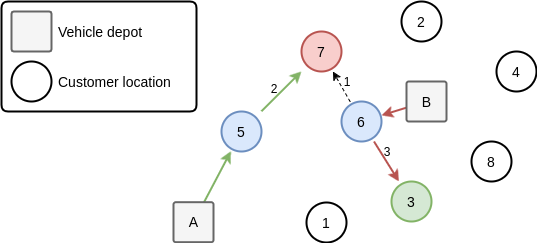
\includegraphics[width=12cm]{Resources/Images/global-best-greedy-solution}
	\captionsetup{format=hang}
	\caption{Ilustrasi \textit{Global Best Solution}}
	\label{fig:global-best-greedy-solution}
\end{figure}


\begin{algorithm}[!]
	\captionsetup{format=hang}
	\caption{\textit{RecommendationPublisher}}
	\label{alg:vrp-worker}
	\begin{algorithmic}[1]
		\renewcommand{\algorithmicrequire}{\textbf{Input:}}
		\renewcommand{\algorithmicensure}{\textbf{Output:}}
		\REQUIRE $TP$		// threadpool
		\ENSURE  $None$
		
		\WHILE {true}
		\STATE $T$ = popFirstThreadOrWaitNewThreadFromThreadpool()
		\STATE $R$ = VRPSolver($T$)
		\FOR {$j = 1$ to $len(R)$}
		\STATE $r$ = publish($C_{R_j}$, $R_j$)
		\IF {($r > 0$)}
		\STATE cancelSolver($T_j$)
		\ELSIF {($C_{T_i} \notin C_{R_j}$)}
		\STATE $T_i = Thread(C_{T_i}, V_m, (unassigned) E_1...E_N)$
		\ENDIF
		\ENDFOR
		\ENDWHILE	
	\end{algorithmic}
\end{algorithm}


Jumlah rute yang dihasilkan oleh \textit{VRPSolver} akan berkisar antara 1 (satu) hingga $M$ rute, dimana $M$ merujuk pada jumlah seluruh petugas pencacahan yang diikutsertakan dalam kalkulasi rute. Setiap rute $R_m$ $(1 \leq m \leq M)$ yang dihasilkan oleh \textit{VRPSolver} akan dikirimkan kepada petugas $m$ yang merupakan \textit{subscriber} topik (lokasi) $C_n$ $(1 \leq n \leq N)$. \textit{Message broker} kemudian akan melaporkan status pengiriman informasi kepada \textit{publisher} (\textit{`success'} atau \textit{`failed'}). Mekanisme kerja \textit{publisher} rekomendasi diilustrasikan dengan menggunakan \textit{flowchart} pada \autoref{fig:recommendation-publisher}.


\begin{figure}[!]
	\centering
	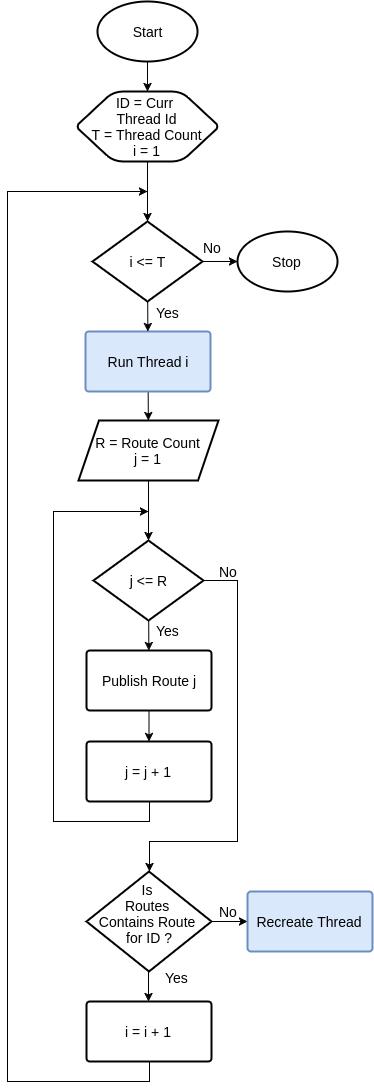
\includegraphics[width=8cm]{Resources/Images/recommendation-publisher}
	\captionsetup{format=hang}
	\caption{\textit{Flowchart recommendation publisher}}
	\label{fig:recommendation-publisher}
\end{figure}


\autoref{fig:timeline-illustration} memberikan gambaran umum tentang proses yang terjadi sejak permintaan lokasi dikirim oleh petugas hingga solusi/rute diperoleh. Petugas B mengirimkan permintaan yang diterima oleh \textit{message broker}. \textit{TopicWatcher} yang memantau \textit{message broker} mengetahui keberadaan permintaan baru ini dan kemudian melaporkannya kepada \textit{publisher}. \textit{Publisher} kemudian menciptakan sebuah \textit{thread} yang mengandung \textit{VRPSolver procedure}. Saat \textit{thread} dieksekusi, \textit{VRPSolver procedure} akan melakukan kalkulasi solusi/rute terbaik dengan mengikutsertakan seluruh $M$ petugas dan lokasi yang masih berstatus \textit{unassigned}. \textit{Thread} hanya dapat dijalankan secara berurutan berdasarkan prinsip `satu dalam satu waktu' (\textit{once at a time}). Sebagai konsekuensinya, ketika petugas A mengirimkan \textit{request} baru, \textit{thread} untuk \textit{request} A tetap akan diciptakan, namun dibiarkan dalam status \textit{idle}. \textit{Thread} A harus menunggu hingga \textit{thread} sebelumnya (\textit{thread} B) selesai diproses. 

Saat \textit{thread} B selesai diproses, \textit{thread} B tidak hanya menghasilkan rute untuk petugas B, tapi juga untuk sejumlah $m$ petugas lainnya ($1 \leq m \leq M$). Rute-rute ini akan dikirimkan kepada petugas yang bersesuaian. Jika suatu rute $R_m$ berhasil diterima oleh petugas $m$, maka \textit{thread} yang berasosiasi dengan rute tersebut akan dihentikan (\textit{terminate}). Dalam \autoref{fig:timeline-illustration}, \textit{thread} B menghasilkan solusi/rute untuk petugas A dan B dan kedua rute ini berhasil diterima dengan baik oleh masing-masing petugas. Dalam hal ini, \textit{thread} A dan \textit{B} dinilai tidak lagi dibutuhkan sehingga kedua \textit{thread} tersebut akan dihentikan. Penghentian ini dilakukan untuk mencegah terjadinya penghitungan ganda terhadap rute yang sudah diterima oleh \textit{subscriber} (petugas). 


\begin{figure}[!]
	\centering
	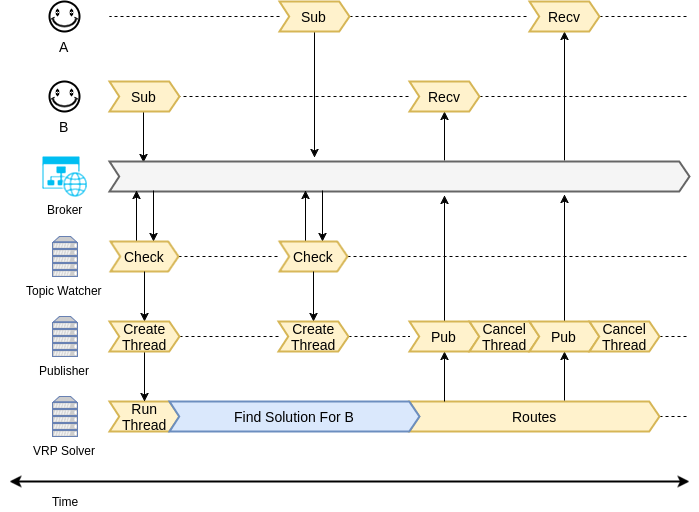
\includegraphics[width=\textwidth]{Resources/Images/timeline-illustration}
	\captionsetup{format=hang}
	\caption{Ilustrasi \textit{Timeline} Proses Pencarian Solusi Berdasarkan}
	\label{fig:timeline-illustration}
\end{figure}


Pada praktiknya, dapat terjadi suatu kondisi dimana \textit{VRPSolver procedure} gagal mendapatkan rute untuk petugas B. Pada kondisi demikian, \textit{thread} B akan diproses ulang dengan hanya melibatkan 1 (satu) petugas B saja dan sejumlah lokasi yang masih berstatus \textit{unassigned}. Ini dilakukan untuk memberikan jaminan bahwa akan selalu ada solusi/rute untuk setiap \textit{request}. 


Pada \autoref{ssec:pub-sub-mechanism} dijelaskan bahwa karakteristik \textit{loose coupling} pada mekanisme \textit{publish/subscribe} membuat \textit{publisher} dan \textit{subscriber} mampu berkomunikasi secara fleksibel, tanpa perlu mengetahui identitas masing-masing. Namun kondisi ini mengakibatkan informasi mengenai `lokasi terkini' dari \textit{subscriber} tidak dapat diperoleh. Untuk mengatasi hal ini, sistem dirancang dengan menyertakan \textit{shared memory}, dimana \textit{subscriber} dapat `menaruh' \textit{current location}-nya agar kemudian dapat  diakses oleh \textit{publisher}. 


%Proses di atas akan terus berulang sampai seluruh lokasi telah di\textit{assign} kepada \textit{subscriber}. \autoref{fig:publisher-algorithm} mengilustrasikan \textit{workflow} dari algoritma yang digunakan pada \textit{recommendation publisher}.
%
%
%\begin{figure}[!]
%	\centering
%	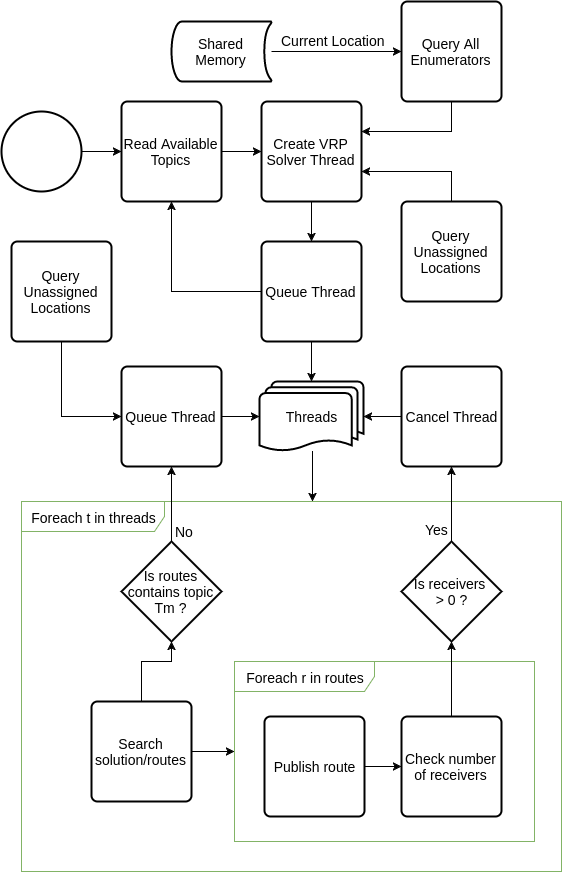
\includegraphics[width=12cm]{Resources/Images/publisher-algorithm}
%	\caption{Publisher Workflow}
%	\label{fig:publisher-algorithm}
%\end{figure}


%-----------------------------------------------------------------------------%
\subsection{\textit{VRP Solver}}
\label{ssec:vrp-solver}
%-----------------------------------------------------------------------------%
\textit{VRP Solver} merupakan sebuah modul yang terdapat di dalam \textit{thread} dan digunakan untuk melakukan kalkulasi rute yang harus dikunjungi oleh petugas. \textit{VRP Solver} dibangun berdasarkan algoritma MDVRP seperti: \textit{tabu search} \cite{cordeau_tabu_1997}, \textit{adaptive large neighborhood search}  \citep{pisinger_general_2007}, \textit{fuzzy logic guided genetic algorithm} \citep{lau_application_2010}, \textit{paralel iterated tabu search} \citep{cordeau_parallel_2012}, \textit{hybrid algorithm combining iterated local search and set partitioning} \citep{subramanian_hybrid_2013}, \textit{hybrid genetic algorithm with adaptive diversity control} \citep{vidal_implicit_2014}, \textit{hybrid granular tabu search} \citep{escobar_hybrid_2014}, dan \textit{cooperative coevolution algorithms} (CoEAs) \citep{de_oliveira_cooperative_2016}. Pada penelitian ini \textit{cooperative coevolutionary algorithms} (CoEAs) dipilih karena menghasilkan rute dengan biaya total yang minimum dan waktu pemrosesan yang relatif singkat dibandingkan algoritma yang lain.


Langkah-langkah yang digunakan dalam implementasi algoritma CoEAs pada \textit{VRPSolver} adalah sebagai berikut:
\begin{enumerate}
\item Definisi masalah \\
Masalah didefinisikan sebagai kumpulan informasi tentang sejumlah $M$ petugas, $N$ lokasi pencacahan, dan $D$ \textit{initial location/depot}. Setiap lokasi $i$, dimana $i \in (D \cup N)$, dilengkapi dengan koordinat lokasi $(x_i, y_i)$. Setiap pasangan lokasi $i$ dan $j$, dimana $i, j \in (D \cup N)$, memiliki biaya sebesar $c_{ij}$ yang merepresentasikan waktu yang diperlukan untuk melakukan perjalanan dari $i$ ke $j$. 

\item Dekomposisi masalah \\
Masalah yang telah didefinisikan sebelumnya akan didekomposisi (dipecah) menjadi beberapa \textit{chunk} submasalah agar proses kalkulasi rute dapat dilakukan secara paralel. 

\item Evolusi \\
Setiap submasalah berisi kombinasi pasangan petugas dan lokasi yang akan dikunjungi (\textit{enumerator-locations pair}). Setiap kombinasi akan mengalami proses evolusi. Pada setiap evolusi yang terjadi, susunan formasi pasangan petugas dan lokasi mengalami perubahan untuk menemukan formasi yang lebih baik. Evolusi terjadi secara iteratif dan setiap iterasi akan menghasilkan formasi baru (\textit{new best formation}). \textit{New best formation} ini akan dievaluasi dengan cara membandingkannya dengan formasi terbaik yang diperoleh dari iterasi sebelumnya (\textit{current best formation}). Jika \textit{new best formation} lebih baik daripada \textit{current best formation}, maka \textit{current best formation} akan diganti dengan \textit{new best formation}. Iterasi akan terus berlangsung sampai dengan solusi/rute yang diperoleh konvergen, yaitu ketika tidak ada lagi \textit{new best formation} yang terbentuk. Formasi yang diperoleh pada akhir keseluruhan iterasi akan dipilih oleh \textit{VRP Solver} sebagai solusi final. 
\end{enumerate}


%-----------------------------------------------------------------------------%
\subsection{\textit{Message Broker}}
\label{ssec:message-broker}
%-----------------------------------------------------------------------------%
\textit{Message broker} merupakan subsistem yang bertanggung jawab dalam menyalurkan (\textit{routing}) pesan dari \textit{publisher} ke \textit{subscriber} dan sebaliknya sesuai dengan topik yang di-\textit{subscribe} \citep{banavar_efficient_1999}. Suatu mekanisme \textit{publish/subscribe} dapat memiliki \textit{single broker} maupun \textit{multi broker}. Pada arsitektur \textit{single broker}, seluruh \textit{subscriber} dan \textit{publisher} terkoneksi pada satu \textit{broker}, sementara pada \textit{multi broker}, \textit{subscriber} maupun \textit{publisher} dapat terkoneksi pada \textit{broker} terdekat. Arsitektur \textit{multi broker} ini disebut juga dengan istilah \textit{distributed publish/subscribe system} \citep{muhl_large-scale_2002}, seperti ilustrasi pada \autoref{fig:pub_sub_distributed_ilustration}. Sistem yang diusulkan akan menerapkan arsitektur terdistribusi agar dapat menangani lokasi pencacahan yang tersebar secara geografis.


\begin{figure}[!]
	\centering
	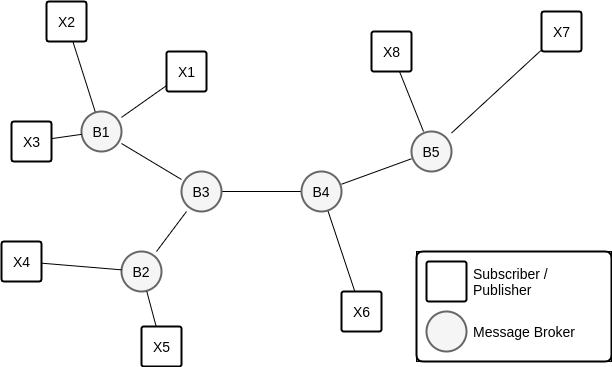
\includegraphics[width=11cm]{Resources/Images/pub_sub_distributed_ilustration}
	\captionsetup{format=hang}
	\caption{Ilustrasi \textit{Publish-Subscribe} terdistribusi}
	\label{fig:pub_sub_distributed_ilustration}
\end{figure}


%#############################################################################%
\begin{comment}
%-----------------------------------------------------------------------------%
\subsection{\textit{Search Algorithm}}
%-----------------------------------------------------------------------------%
Terdapat berbagai variasi algoritma untuk menyelesaikan permasalah TSP maupun VRP, antara lain: genetic algorithm, simmulated annealing, tabu search, particle swarm optimization, harmony search, quantum annealing, greedy 2-opt, dll. Pada pengujian yang dilakukan dengan kasus single-salesman dengan menggunakan 3 (tiga) kriteria: \textit{mean quality}, \textit{dispersion of quality}, dan \textit{time needed to reach the optimum}, simmulated annealing menghasilkan solusi yang paling berkualitas, sementara tabu search merupakan yang paling baik dari sisi performance \citep{antosiewicz_choice_2013}.


%-----------------------------------------------------------------------------%
\subsection{\textit{Greedy Strategy}}
%-----------------------------------------------------------------------------%
Algoritma \textit{greedy} adalah suatu algoritma yang menentukan solusi optimal berdasarkan kondisi saat ini, atau disebut dengan \textit{local optimum}. Algoritma greedy dapat meminimalisir waktu komputasi dalam pencarian solusi global. Pada kasus \textit{travelling salesman problem}, strategi greedy dapat dikatakan dengan "pada setiap tahap, kunjungi kota yang paling dekat dengan lokasi salesman yang belum dikunjungi" \citep{paul_e._black_greedy_2005}. 


Pada metode MTSP, diperoleh lebih dari satu solusi, dimana masing-masing solusi diperbandingkan. Perbandingan dilakukan berdasarkan biaya keseluruhan, dimana solusi dengan biaya terkecil adalah solusi terbaik.


Penentuan solusi terbaik dengan membandingkan biaya keseluruhan tidaklah tepat. \textit{Cost} ditentukan dengan satuan waktu, sementara salah satu komponen utama yang dominan adalah \textit{service time}. Karena \textit{service time} tidak tersedia, maka membandingkan keseluruhan waktu akan menjadi bias. Hipotesis yang ditawarkan adalah membandingkan setiap solusi dengan total biaya untuk lokasi pertama dari masing-masing pencacah saja, karena lokasi pertama tidak terpengaruh dengan \textit{service time}, seperti algoritma dalam Kode \ref{lst:proposed_best_solution_algorithm}.


\begin{listing}
	\caption{Algoritma Solusi Terbaik}
	\label{lst:proposed_best_solution_algorithm}
	\begin{minted}[showspaces=false,breaklines=true]{python}
Let E be all enumerators
Let L be all locations
Run MTSP with enumerators E and locations L
Let S be all solutions from MTSP
Let Cs be an empty dict
For each solution s in S do
	Let R be all routes in solution s
	Let C be 0
	For each route r in R do
		Let J be all jobs in route r
		Let fj be first job in J
		Let cfj be cost of first job fj
		Add C with cjf
	Put C in dict Cs with key solution s
	
Let element in dict Cs with the least value be the best solution
	\end{minted}
\end{listing}


Algoritma \ref{lst:proposed_best_solution_algorithm} merupakan rekomendasi lokasi pertama untuk setiap pencacah. Selanjutnya pencacah dapat melakukan pengumpulan data pada lokasi tersebut sampai selesai, dengan \textit{service time} bervariasi, sehingga waktu selesai pencacahan berbeda-beda antar pencacah. Setiap pencacah yang telah menyelesaikan pengumpulan data, dapat melakukan \textit{subscribe} solusi yang baru kepada \textit{broker}, seperti algoritma pada Kode \ref{lst:proposed_subscribe_solution_algorithm}. Setiap kali broker mendapati adanya \textit{subscribers}, maka \textit{broker} akan mencari solusi baru dengan metode MTSP. Solusi yang dicari hanya menyertakan \textit{subscribers} saja, dan meng-\textit{exclude} lokasi yang telah dikunjungi, seperti algoritma pada Kode \ref{lst:proposed_subscribers_best_solution_algorithm}.


\begin{listing}
	\caption{Algoritma \textit{Subscribe Solution}}
	\label{lst:proposed_subscribe_solution_algorithm}
	\begin{minted}[showspaces=false,breaklines=true]{python}
Let SS be an empty list
For each e in enumerators E do
	If enumerator e has finished enumerating do
		Exclude location l enumerated by e from locations L
		Add e in list of subscribers SS
	\end{minted}
\end{listing}


\begin{listing}
	\caption{Algoritma Solusi Terbaik untuk \textit{Subscribers}}
	\label{lst:proposed_subscribers_best_solution_algorithm}
	\begin{minted}[showspaces=false,breaklines=true]{python}
While locations L is not empty do
	Run MTSP with enumerators SS and locations L
    Let S be all solutions from MTSP
    Let Cs be an empty dict
    For each solution s in S do
	    Let R be all routes in solution s
	    Let C be 0
	    For each route r in R do
		    Let J be all jobs in route r
		    Let fj be first job in J
		    Let cfj be cost of first job fj
		    Add C with cjf
	    Put C in dict Cs with key solution s
	
    Let Bs as element in dict Cs with the least value
    Publish Bs to all subscribers SS
    Set subscribers SS to empty list
	\end{minted}
\end{listing}


%-----------------------------------------------------------------------------%
\subsection{\textit{Publish/Subscribe Paradigm}}
%-----------------------------------------------------------------------------%








\section{Garis Besar Perancangan}

Alur kerja perancangan dimulai dengan dengan mengidentifikasi blok sensus yang akan dilakukan pendataan padanya, serta menentukan jumlah pencacah yang akan digunakan. Kedua permasalahan ini tidak akan dibahas terlalu mendalam dalam penelitian ini. Lokasi pencacahan telah ditentukan dalam fase perancangan sensus dan survei, mengikuti sebuah metodologi tertentu. Sementara jumlah pencacahan juga telah ditentukan, mengikuti jumlah sampel dan berbagai persyaratan tertentu, seperti waktu dan biaya.


Selanjutnya, setiap pencacah akan dialokasikan kepada blok sensus yang akan dicacah dengan menggunakan metode MTSP, sebagaimana diformulasikan oleh \citep{bektas_multiple_2006}, dengan ketentuan setiap pencacah dapat memulai dan mengakhiri pada depot yang berbeda-beda. Setelah model diperoleh, setiap pencacah akan mengunjungi lokasi pertama dari rekomendasi. Setelah selesai kunjungan, lokasi akan disimpan dalam \textit{tabu list} dengan menggunakan metode pub-sub \citep{chen_efficient_2003}. Model baru akan digenerate setiap kali terdapat \textit{request} dari salah satu pencacah. Setiap kali model di-\textit{generate}, \textit{tabu search} \citep{glover_tabu_1989, glover_tabu_1990} yang memanfaatkan \textit{tabu list} akan digunakan untuk memastikan tidak terdapat \textit{conflict}. Setelah model baru selesai di-\textit{generate}, maka mudel akan di-\textit{publish} kepada setiap pencacah yang telah men-\textit{subscribe}.


\begin{figure}[!]
    \centering
    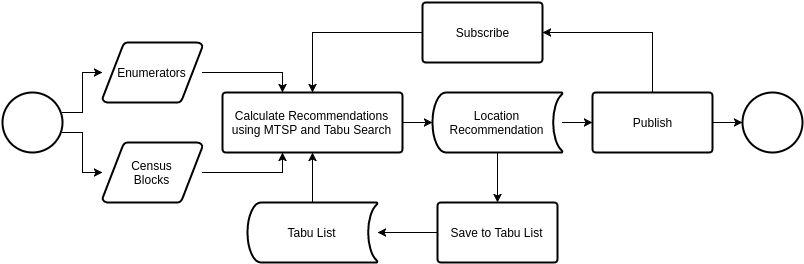
\includegraphics[width=\textwidth]{Resources/Images/design_overview}
    \caption{Garis Besar Sistem Usulan}
    \label{fig:design_overview}
\end{figure}


\section{Penyusunan Rekomendasi}

Pada tahap perumusan rekomendasi, input data yang terdiri dari data pencacah dan data blok sensus akan dioleh menjadi rekomendasi path yang harus dikunjungi. Proses penyusunan rekomendasi menggunakan metode \textit{Multiple Travelling Salesman Problem} (MTSP), yang merupakan pengembangan dari metode klasik \textit{Travelling Salesman Problem} (TSP).


Metode MTSP yang digunakan dalam masalah ini memiliki beberapa \textit{requirements}, antara lain:

\begin{itemize}
\item Jumlah depot \\
MTSP dapat menggunakan lebih dari satu depot, dengan $ m_{j} $ \textit{salesman} untuk setiap depot $ j $. Pada permasalahan ini menggunakan \textit{non-fixed destination}, sehingga pencacahan tidak perlu kembali ke lokasi dimana pencacahan dimulai.
\item Jumlah \textit{salesman} \\
Jumlah \textit{salesman} yang digunakan dapat berupa \textit{fixed number} $ m $, atau dinamis dengan dibatasi jumlah maksimal $ max(m) $. Pada permasalahan ini digunakan \textit{fixed number} $ m $ pencacah.
\item \textit{Fixed charges} \\
Jika jumlah \textit{salesman} dinamis, maka bisa juga masing-masing \textit{salesman} dibatasi dengan sejumlah biaya tertentu. Pada permasalahan ini tidak digunakan \textit{fixed charges}.
\item Waktu kunjungan (\textit{time windows}) \\
\textit{Time windows} merepresentasikan waktu yang dihabiskan selama kunjugan dalam sebuah \textit{node}. Pada kasus ini \textit{time windows} tidak dapat ditentukan karena tidak tersedianya informasi, sehingga dianggap tidak menggunakan \textit{time windows}.
\end{itemize}


Requirements di atas, secara global dapat disederhanakan dalam tabel-tebel berikut. Tabel \ref{tbl:enumerators_overview} menunjukkan rancangan pencacah beserta koordinat depot-nya, sementara Tabel \ref{tbl:census_blocks} menunjukkan rancangan blok sensus beserta koordinat dan \textit{time windows}-nya. Dalam fakta lapangan, jarak antara satu blok sensus dengan blok sensus yang lain tidaklah setara. Bisa jadi secara koordinat memiliki jarak yang berdekatan, tetapi secara akses tidaklah mudah. Untuk itu diperlukan sebuah tabel tambahan, yaitu tabel \textit{cost-matrix}, sebagaimana Tabel \ref{tbl:cost_matrix}. \textit{Cost} yang dimaksud disini adalah segala metrik yang dapat digunakan sebagai penimbang (\textit{weight}), misalnya: biaya, jarak, atau waktu tempuh.


\begin{table}[]
\centering
\caption{Table Pencacah}
\label{tbl:enumerators_overview}
\begin{tabular}{@{}lcc@{}}
\toprule
\multirow{2}{*}{Pencacah} & \multicolumn{2}{l}{\textit{Depot Coordinate}} \\ \cmidrule(l){2-3} 
                          & X                 & Y                \\ \midrule
Pencacah 1                & 20.0              & 20.0             \\
Pencacah 2                & 20.0              & 20.0             \\
Pencacah 3                & 30.0              & 40.0             \\
Pencacah 4                & 30.0              & 40.0             \\
...                       &                   &                  \\
Pencacah m                & x                 & y                \\ \bottomrule
\end{tabular}
\end{table}


\begin{table}[]
\centering
\caption{Tabel Blok Sensus}
\label{tbl:census_blocks}
\begin{tabular}{@{}lccc@{}}
\toprule
\multirow{2}{*}{Blok Sensus} & \multicolumn{2}{c}{Koordinat Lokasi} & \multirow{2}{*}{Time Windows} \\ \cmidrule(lr){2-3}
                             & X                 & Y                &                               \\ \midrule
001B                         & 62.0              & 63.0             & 0                             \\
002B                         & 63.0              & 69.0             & 0                             \\
003B                         & 46.0              & 10.0             & 0                             \\
004B                         & 61.0              & 33.0             & 0                             \\
...                          &                   &                  &                               \\
n                            & x                 & y                & 0                             \\ \bottomrule
\end{tabular}
\end{table}


\begin{table}[]
\centering
\caption{Table \textit{Cost-Matrix}}
\label{tbl:cost_matrix}
\begin{tabular}{@{}|c|c|c|c|c|c|c|@{}}
\toprule
        & 001B & 002B & 003B & 004B & ... & BS ke-n \\ \midrule
001B    & -    & 5    & 2    & 2    &     & ...     \\ \midrule
002B    &      & -    & 4    & 2    &     & ...     \\ \midrule
003B    &      &      & -    & 7    &     & ...     \\ \midrule
004B    &      &      &      & -    &     & ...     \\ \midrule
...     &      &      &      &      & -   & ...     \\ \midrule
BS ke-n &      &      &      &      &     & -       \\ \bottomrule
\end{tabular}
\end{table}


Tabel \textit{cost-matrix}, selain dapat didefinisikan secara manual (berdasarkan hasil survei atau perkiraan \textit{subject matter}), dapat juga didekati dengan menggunakan Google Directions API \citep{google_google_2016}. \textit{Request} yang digunakan menggunakan standar REST API, sementara \textit{response} yang ditampilkan dalam format JSON. Listing \ref{lst:google_direction_api_request} menunjukkan contoh \textit{request}, dan Gambar \ref{fig:google_direction_api_response} menunjukkan contoh \textit{response} dari Google Direction API.








%Gambar \ref{fig:mtsp_solution_example} berikut menunjukkan hasil rekomendasi dengan MTSP.
%
%
%\begin{figure}[!]
%    \centering
%    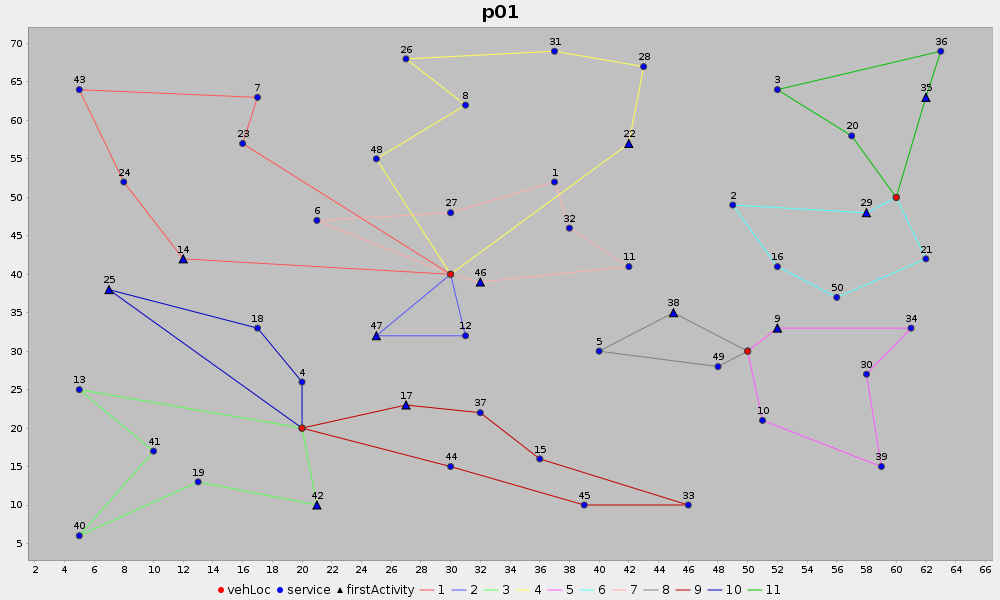
\includegraphics[width=\textwidth]{Resources/Images/mtsp_solution_example}
%    \caption{Contoh Hasil Rekomendasi}
%    \label{fig:mtsp_solution_example}
%\end{figure}


\section{Penyusunan \textit{Conflict Resolution}}


\section{\textit{Publish-Subscribe} Rekomendasi}
\end{comment}
%#############################################################################%
